\documentclass[conference,10pt]{IEEEtran}
\IEEEoverridecommandlockouts
\usepackage{graphicx,booktabs,amsmath,amssymb,multirow,xcolor,url,xspace}
\usepackage[hidelinks]{hyperref}
\hypersetup{pdftitle={로봇 양팔을 위한 에고센트릭 인간 시연, 제2부: 단일 팔 큐브 접근(Approach)}, pdfauthor={Jeong Hwan Lee}}
\usepackage{tikz}
\usetikzlibrary{positioning,arrows.meta,fit,backgrounds}
\usepackage{fontspec}\setmainfont{Times New Roman}\usepackage{xeCJK}\setCJKmainfont[AutoFakeBold=1.5]{AppleMyungjo}\setCJKsansfont{Apple SD Gothic Neo}\setCJKmonofont{Apple SD Gothic Neo}\xeCJKsetup{CJKecglue={},CJKspace=true}
\newcommand{\mm}{\,mm\xspace}

\begin{document}
\title{로봇 양팔을 위한 에고센트릭 인간 시연\\제2부: 단일 팔 큐브 접근(Approach)}
\author{\IEEEauthorblockN{Jeong Hwan Lee}
\IEEEauthorblockA{기술 보고서, 버전 4, 2026년 10월 7일 \quad alnrg2arg@gmail.com\\
요약본. 제1부는 큐브 삼단 쌓기를 다룹니다. 코드, 결과, 샘플 데이터는 요청 시 제공합니다.}}
\maketitle

\begin{abstract}
전이 가능한 가장 단순한 행동, 즉 에고센트릭 인간 시연만으로 학습한 오른팔의 빨간 큐브 접근을 따로 떼어 다룬다. 이러한
느린 동작에서는 IMU 시각-관성 스케일이 관측 불가능하므로, 스케일은 3.8\,cm 큐브 또는 테이프 원점에서의 테이블 평면으로부터
얻는다. 공유 작업 좌표계, 로봇 손목 핸드-아이 보정(0.16\,px RMS), 로봇 카메라 렌더링을 통해 인간 레이블을 로봇 좌표계에
놓는다. 80--150개 테이크로 학습한 모델은 첫 체크포인트부터 과적합한다. 로봇 실행에서는 정지 사유만 기록되고 결과는
기록되지 않았으므로 성공률은 보고하지 않는다.
\end{abstract}

\section{실험 구성}
작업자는 오른손에 HandUMI~\cite{chi2024umi} 한 대(손목 어안 카메라, IMU, 조 엔코더)를 착용하며, 손목 자세는
MASt3R-SLAM~\cite{murai2025mast3rslam}에서 얻는다(제1부). 레이블은 제1부의 데카르트 계약(50.05\,ms 간격의 상대 자세 16개,
15\,Hz 행)을 따른다. 왼팔과 그리퍼는 더미로서 손실에서 마스킹되므로 20차원 중 9차원만 지도된다. 모델은 X-VLA
(0.9B)~\cite{zheng2025xvla}이며 제1부의 레시피(소프트 프롬프트 슬롯 20, 배치 8, 8-bit AdamW, bf16)로 RTX~4090에서 학습한다.
로봇은 손목 C922가 달린 reBot B601 오른팔이며, 배포 중에는 왼팔과 양쪽 조를 잠근다.

\section{IMU 없이 얻는 미터 스케일}
\textbf{HRA\_red.} 10월 3일 ``빨간 큐브에 접근'' 테이크 200개(10\,s)를 녹화했다. 에피소드별 IMU 스케일은 중앙값이
0.012이고 95개 테이크에서 0 또는 음수이다(그림~\ref{fig:cube}b). 느린 접근은 가속도계를 충분히 자극하지 못한다.
\textbf{큐브 PnP.} 정지한 큐브(모서리 3.8\,cm)를 2면/3면 모델 또는 정면에 가까운 단일 면 모델로 피팅하고, 큐브가 움직이지
않는다는 조건으로부터 궤적 스케일을 닫힌 형태로 구한다. IMU를 신뢰할 수 있는 양손 HRL80 테이크에서는 57개 중 37개가 PnP
유효이며 PnP/IMU 비는 1.062(p16--p84 0.959--1.274; 그림~\ref{fig:cube}a)이다. 스케일 게이트와 타당성 게이트를 거쳐 200개 중
166개 테이크가 남는다(학습 151개, 20{,}319행; 검증 15개). 스케일 중앙값은 0.354(p5 0.188, p95 0.500), 큐브 중심 잔차는
0.17\,cm이다.

\begin{figure*}[t]
\centering
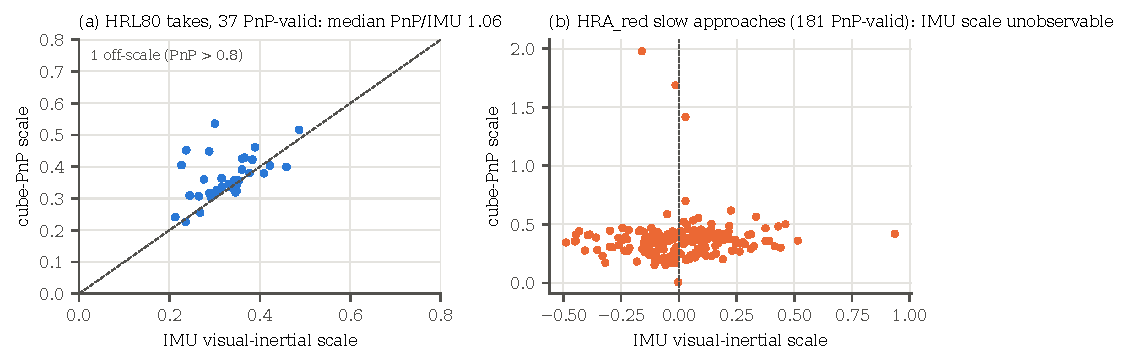
\includegraphics[width=0.78\textwidth]{figures/fig6_cube_scale.pdf}
\caption{IMU와 큐브 PnP로 구한 테이크별 미터 스케일. (a) IMU를 신뢰할 수 있는 HRL80 쌓기 테이크. (b) HRA\_red 접근
테이크: IMU 스케일이 0 주변에 흩어진다.}
\label{fig:cube}
\end{figure*}

\section{인간 데이터를 로봇 좌표계에 놓기}
\textbf{로봇 보정.} 헤드 C922를 체커보드로 보정하고(RMS 1.05\,px), 보드 모서리를 터치하여 로봇 베이스에서의 위치를 구했다.
로봇 손목 카메라의 핸드-아이 보정(뷰 13장, 0.16\,px RMS)에 따르면 카메라는 TCP보다 169.5\mm{} 뒤에 있으며, 광축은 TCP $x$축보다
33\textdegree{} 아래를 향한다. IK 스택의 TCP는 실제 조 끝단보다 약 82\mm{} 앞에 있다. 이제 접촉은 URDF 손끝 박스로 판정하며,
이전의 ``끝단이 테이블 아래로 내려간다''는 판독은 이 인공물 때문이었으므로 철회했다. HRA\_red 테이크를 헤드 카메라를 통해
사후에 베이스와 연결한 결과는 166개 중 64개에 그쳤고 높이가 센티미터 단위로 퍼졌으며, 내보낸 카메라--IMU 외부 파라미터의
18\textdegree{} 오류가 드러났다.

\textbf{로봇 카메라 렌더링(v2).} v1은 추정한 카메라(화각 62--70\textdegree)로 손목 뷰를 렌더링했다. v2는 실측한 로봇
카메라(52\textdegree)와 핸드-아이 자세를 사용하고, 레이블을 로봇 TCP 자세로 표현한다.

\textbf{공유 원점(HRA\_A100).} 각 테이크는 로봇 조 끝단도 터치했던 테이프 십자 위에 HandUMI 조 끝단을 2\,s 동안 대는
것으로 시작하며, 이어 3\,s 동안 로봇과 비슷한 시작 자세로 옮기고 10\,s 동안 접근한다. 테이프 선 위의 로봇 터치 세 점이
작업 좌표계 G를 정의한다(60.4\mm{}에 걸쳐 0.38\mm{} 이내로 공선, 테이블은 $z=-27.1$\mm). 원점에서는 첫 MASt3R 포인트맵의
테이블 평면이 두 번째 스케일 원천이 되며(큐브 PnP 대비 비 0.999, 테이크별 오차 p50 8\%, p90 37\%), 원점 yaw는 테이크마다
측정한다(오차 p50 0.21\textdegree). 10월 6일 107개 테이크를 확보했다. 테이블 인지 변환(손끝 하한은 테이블 + 5\mm, 끝점
들어올림은 최대 30\mm)은 86개를 유지하며(CT5/CT6), 손끝 여유는 p50 12.6\mm, 최소 7.6\mm{}이다.

\section{학습}
\begin{table}[t]
\centering\footnotesize\setlength{\tabcolsep}{4pt}
\caption{체크포인트별 held-out 손실(마스킹된 MSE). 괄호 안은 학습 부분집합 손실.}
\label{tab:val}
\resizebox{\columnwidth}{!}{\begin{tabular}{@{}lccc@{}}
\toprule
데이터(검증 테이크) & 첫 체크포인트 & 중간 & 마지막 평가 \\
\midrule
HRA\_red v1 (15) & 15k: 0.150 (0.066) & 30k: 0.198 & 105k: 0.299 (0.018) \\
A100, 시작점 기준 (11) & 5k: 0.124 (0.110) & 30k: 0.141 & 50k: 0.224 (0.020) \\
A100, 원점 기준 (11) & 5k: 0.132 (0.097) & 30k: 0.174 & 45k: 0.190 (0.022) \\
\bottomrule
\end{tabular}}
\end{table}
모든 실행은 처음 평가한 체크포인트부터 과적합하며(표~\ref{tab:val}), v1 300k 실행은 학습 손실 0.002로 끝났다. 상태의
기준을 테이크 시작점에 두든 원점에 두든 held-out 손실에는 차이가 없다. 이 글을 쓰는 시점에는 10월 6일 채택 테이크 85개와
선택한 로봇 시작 자세를 사용한 실행(CT7)이 진행 중이었다.

\section{로봇 실행과 배포}
v1은 가까운 시작점에서는 큐브를 향해 움직였고, 먼 큐브에 대해서는 테이블 위를 끌며 이동했다(두 번의 실행에서 각각 약 39\,cm,
26\,cm). 10월 7일 작업자가 팔이 큐브를 미는 것을 관찰하여, 이제 인터페이스는 손목 뷰에서 큐브의 겉보기 크기가 임계값을
넘으면 정지한다(근접 대리 지표이지 검증된 접촉이 아니다). 그날 127개 세션 중 69개가 이렇게 끝났다. 실행 설정은
체크포인트만큼 중요했다. 인터페이스 재시작으로 청크 블렌딩 파라미터가 조용히 초기화되자, 작업자는 값을 복원할 때까지
추론 품질이 “많이 낮아졌다”고 보고했다. 시행 결과는 기록되지 않았으므로 성공률은 없다.

\section{교훈과 향후 과제}
모든 스케일 원천은 어딘가에서 조용히 실패하므로(느린 동작에서의 IMU, 일부 테이크에서의 원점 평면) 독립적인 원천이 두 개
필요하다. 로봇과 공유하는 물리적 원점이 사후 정합보다 낫다. IK TCP는 규약일 뿐 손끝이 아니다. 작은 단일 작업 데이터셋은
즉시 과적합하므로 시험할 것은 이른 체크포인트이다. 실행 설정은 정책의 일부이다. 다음 단계는 고정된 시작 자세와 큐브
위치에서 설정을 고정한 채 시행을 기록하는 것, A, B, CT7의 이른 체크포인트를 시험하는 것, 렌더링 이미지의 큐브 색(학습에서는
주황색, 로봇에서는 빨간색)을 보정하는 것이다.

\begin{thebibliography}{9}\footnotesize
\bibitem{chi2024umi} C.~Chi \emph{et al.}, ``Universal manipulation interface,'' in \emph{RSS}, 2024.
\bibitem{murai2025mast3rslam} R.~Murai, E.~Dexheimer, and A.~J. Davison, ``MASt3R-SLAM,'' in \emph{CVPR}, 2025.
\bibitem{zheng2025xvla} J.~Zheng \emph{et al.}, ``X-VLA: Soft-prompted transformer as scalable cross-embodiment VLA model,'' in \emph{ICLR}, 2026.
\end{thebibliography}
\end{document}
